% =====================================================================
% Inkling-turbo, all figures in one self-contained file.
%
% Paste this into Overleaf as a single .tex and compile with pdfLaTeX.
% No other files are needed. You get a 3 page PDF, one cropped figure
% per page:
%     page 1  attention kernel latency
%     page 2  full-model agreement with the stock build
%     page 3  validation status
%
% EVERY number below is measured. Nothing is interpolated or estimated.
% Sources, all in this repository:
%   journal/remote/microbench_attn_day0_session25_h100.json      (ours)
%   journal/remote/microbench_attn_scoremod_session25_h100.json  (day-0)
%   journal/remote/gate_logit_parity_8xh100.json                 (token gate)
% A missing point means that pairing was never run.
%
% Two tikz traps worth knowing, both hit while writing this:
%   1. color= after fill= silently overrides the fill. Use text= instead.
%   2. \foreach does not survive inside a pgfplots axis, because pgfplots
%      replays the axis body at \end{axis}. Row labels belong in
%      yticklabels, values in nodes near coords.
% =====================================================================

\documentclass[border=14pt,multi=tikzpicture]{standalone}
\usepackage{tikz}
\usepackage{pgfplots}
\pgfplotsset{compat=1.18}
\usetikzlibrary{calc,plotmarks}

% ---- palette ----------------------------------------------------------
\definecolor{ours}{HTML}{0B6E6A}     % our kernel
\definecolor{floorc}{HTML}{64748B}   % the biasless floor / controls
\definecolor{prod}{HTML}{C2410C}     % the path vLLM ships
\definecolor{altA}{HTML}{9A3412}     % other day-0 paths
\definecolor{altB}{HTML}{78350F}
\definecolor{ink}{HTML}{111827}      % text
\definecolor{guide}{HTML}{DDE1E6}    % grid
\definecolor{okc}{HTML}{15803D}      % validated
\definecolor{partc}{HTML}{B45309}    % partial

% ---- shared axis look -------------------------------------------------
\pgfplotsset{
  inkling/.style={
    scale only axis,
    axis line style={draw=none},
    tick style={draw=none},
    grid style={line width=0.45pt, color=guide},
    xticklabel style={font=\scriptsize, color=ink!62},
    yticklabel style={font=\scriptsize, color=ink!88},
    xlabel style={font=\footnotesize, color=ink!85},
    clip=false,
  },
}

% ---- title + standfirst above a named axis ----------------------------
\newcommand{\figtitle}[3]{%
  \node[anchor=north west, font=\bfseries, color=ink]
    at ($(#1.north west)+(\titleoffset,\titletop)$) {\large #2};
  \node[anchor=north west, font=\scriptsize, color=ink!58,
        text width=\standfirstwidth]
    at ($(#1.north west)+(\titleoffset,\titlesub)$) {#3};
}

\begin{document}
\sffamily

% =====================================================================
% PAGE 1: attention kernel latency
% =====================================================================
\def\titleoffset{-3.55cm}
\def\titletop{1.75cm}
\def\titlesub{1.30cm}
\def\standfirstwidth{16.6cm}

\begin{tikzpicture}[font=\sffamily]
\begin{axis}[
  inkling,
  name=A,
  width=11.6cm, height=8.8cm,
  xmode=log, log basis x=10,
  xmin=640, xmax=26000,
  xtick={1000,2000,5000,10000,20000},
  xticklabels={1000,2000,5000,{10\,000},{20\,000}},
  xlabel={kernel latency per iteration, microseconds (log scale)},
  ymin=0.35, ymax=15.65,
  ytick={1,2,3,5,6,7,8,9,11,12,13,14,15},
  yticklabels={
    {day-0 relproj},
    {day-0 relproj, transposed},
    {\textbf{Inkling-turbo}},
    {day-0 relproj},
    {day-0 relproj, transposed},
    {day-0 \texttt{score\_mod}},
    {plain attention, no bias},
    {\textbf{Inkling-turbo}},
    {day-0 relproj},
    {day-0 relproj, transposed},
    {day-0 \texttt{score\_mod}},
    {plain attention, no bias},
    {\textbf{Inkling-turbo}}},
  ymajorgrids, xmajorgrids,
  point meta=explicit symbolic,
  nodes near coords,
  nodes near coords style={font=\scriptsize, color=ink!62, anchor=west,
                           xshift=5pt},
]
\addplot[only marks, mark=*, mark size=3.4pt, color=ours]
  coordinates {(852.6,15) [853] (854.8,9) [855] (3308.8,3) [3309]};
\addplot[only marks, mark=o, mark size=3.1pt, line width=1.1pt, color=floorc]
  coordinates {(736.0,14) [736] (727.2,8) [727]};
\addplot[only marks, mark=square*, mark size=2.9pt, color=prod]
  coordinates {(2326.6,13) [2327] (2391.2,7) [2391]};
\addplot[only marks, mark=triangle*, mark size=3.7pt, color=altA]
  coordinates {(5154.7,12) [5155] (5065.1,6) [5065] (10551.5,2) [10552]};
\addplot[only marks, mark=diamond*, mark size=3.7pt, color=altB]
  coordinates {(7194.5,11) [7195] (7595.5,5) [7596] (15254.6,1) [15255]};
\end{axis}

\node[anchor=east, font=\footnotesize\bfseries, color=ink, align=right]
  at ($(A.north west)+(-3.45cm,-0.32cm)$)
  {decode, batch 1\\[-2pt]{\scriptsize\mdseries\color{ink!52}64K KV}};
\node[anchor=east, font=\footnotesize\bfseries, color=ink, align=right]
  at ($(A.north west)+(-3.45cm,-3.72cm)$)
  {decode, batch 32\\[-2pt]{\scriptsize\mdseries\color{ink!52}64K KV}};
\node[anchor=east, font=\footnotesize\bfseries, color=ink, align=right]
  at ($(A.north west)+(-3.45cm,-7.12cm)$)
  {prefill, 8K\\[-2pt]{\scriptsize\mdseries\color{ink!52}global}};

\node[anchor=west, font=\scriptsize\bfseries, color=ours]
  at ($(A.north east)+(0.35cm,-1.44cm)$) {2.7x faster};
\node[anchor=west, font=\scriptsize\bfseries, color=ours]
  at ($(A.north east)+(0.35cm,-4.84cm)$) {2.8x faster};
\node[anchor=west, font=\scriptsize\bfseries, color=ours]
  at ($(A.north east)+(0.35cm,-7.68cm)$) {3.2x faster};

\figtitle{A}{Attention kernel latency}{%
  One H100 SXM5. Same machine, same harness, same shapes, and every point has
  a passing parity run behind it. The hollow marker is biasless attention: the
  floor this feature can approach but never beat. Speedups are quoted against
  \texttt{score\_mod}, the path vLLM actually ships, or against the fastest
  day-0 path measured where \texttt{score\_mod} was not run.}
\end{tikzpicture}

% =====================================================================
% PAGE 2: full-model agreement with the stock build
% =====================================================================
\def\titleoffset{-6.15cm}
\def\titletop{1.72cm}
\def\titlesub{1.28cm}
\def\standfirstwidth{16.4cm}

\begin{tikzpicture}[font=\sffamily]
\begin{axis}[
  inkling,
  name=A,
  width=9.4cm, height=3.6cm,
  xbar,
  bar width=14pt,
  xmin=0, xmax=0.185,
  xtick={0,0.05,0.10,0.15},
  xticklabels={0,0.05,0.10,0.15},
  xlabel={mean absolute difference in per-token logprob},
  ymin=-0.8, ymax=2.8,
  ytick={0,1,2},
  yticklabels={
    {\textbf{Inkling-turbo} vs itself},
    {stock day-0 vs itself},
    {\textbf{Inkling-turbo} vs stock day-0}},
  xmajorgrids,
  nodes near coords,
  nodes near coords style={font=\scriptsize, color=ink!72, anchor=west,
                           xshift=3pt, /pgf/number format/fixed,
                           /pgf/number format/precision=3,
                           /pgf/number format/fixed zerofill},
]
\addplot[fill=ours, draw=ours] coordinates {(0.0477,2)};
\addplot[fill=floorc!28, draw=floorc!75] coordinates {(0.1496,1) (0.1628,0)};
\end{axis}

\draw[floorc!75, line width=0.8pt]
  ($(A.north east)+(0.30cm,-1.30cm)$) --
  ($(A.north east)+(0.48cm,-1.30cm)$) --
  ($(A.north east)+(0.48cm,-3.10cm)$) --
  ($(A.north east)+(0.30cm,-3.10cm)$);
\node[anchor=west, font=\scriptsize, color=floorc, align=left]
  at ($(A.north east)+(0.60cm,-2.20cm)$)
  {\textbf{platform noise floor}\\[-1pt]
   {\color{ink!52}the same build,}\\[-2pt]
   {\color{ink!52}disagreeing with itself}};

\node[anchor=west, font=\scriptsize\bfseries, color=ours]
  at ($(A.north east)+(0.60cm,-0.42cm)$) {3.1x below the floor};

\node[anchor=north west, draw=okc!30, fill=okc!7, rounded corners=2.5pt,
      line width=0.7pt, inner sep=9pt, text width=15.7cm, align=left,
      font=\small, text=ink]
  at ($(A.south west)+(-6.15cm,-1.28cm)$)
  {\textbf{\color{okc}32 of 32 prompts produced identical greedy tokens.}
   2369 tokens compared, on the real 975B NVFP4 checkpoint at TP8. Neither
   control reproduced its own tokens across batch sizes, so the platform
   itself is not batch-deterministic at this scale.};

\figtitle{A}{Full-model agreement with the stock build}{%
  8x H100 SXM5, TP8. Both builds served the same checkpoint on the same
  machine with the same seed. The lower two bars are controls: each build
  compared against itself at a different batch size. They set the floor that
  any cross-build number has to be read against.}
\end{tikzpicture}

% =====================================================================
% PAGE 3: validation status
% =====================================================================
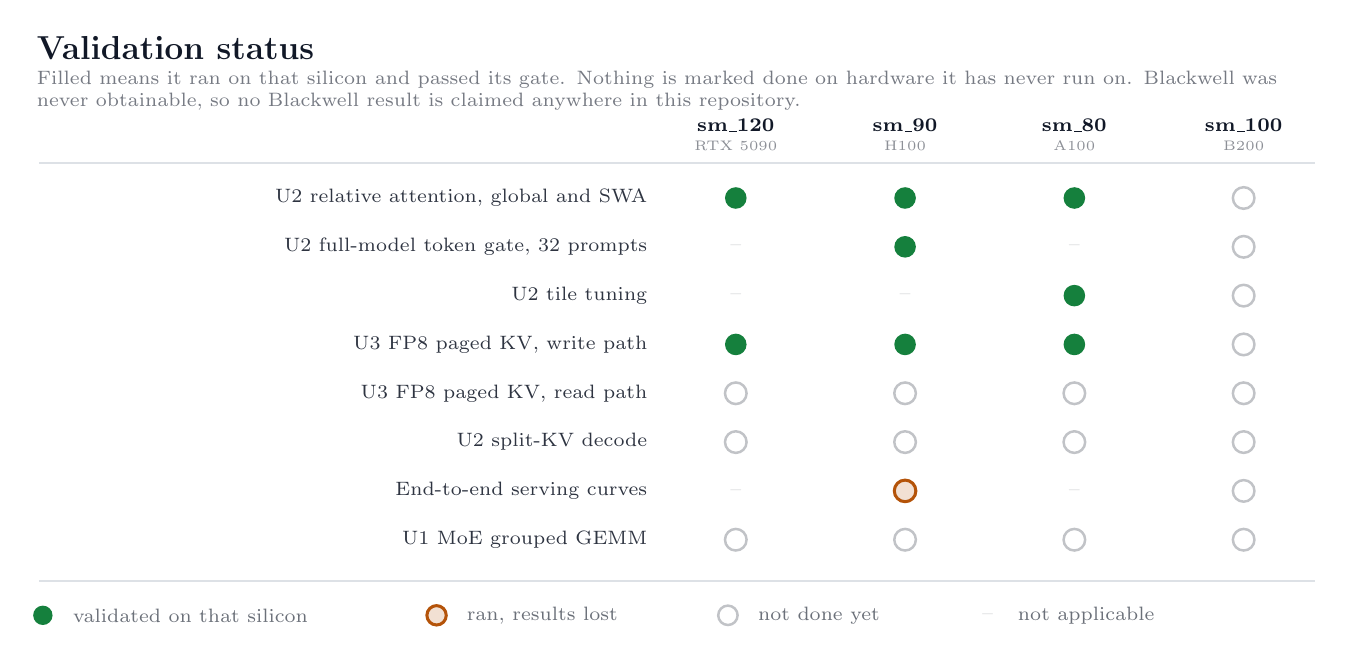
\begin{tikzpicture}[font=\sffamily]

\def\cz{9.0}
\def\cw{2.15}
\def\rh{0.62}
\def\labx{8.0}

\node[anchor=north west, font=\bfseries, color=ink] at (0,1.05cm)
  {\large Validation status};
\node[anchor=north west, font=\scriptsize, color=ink!58, text width=16.2cm]
  at (0,0.62cm)
  {Filled means it ran on that silicon and passed its gate. Nothing is marked
   done on hardware it has never run on. Blackwell was never obtainable, so
   no Blackwell result is claimed anywhere in this repository.};

\node[font=\scriptsize\bfseries, color=ink] at (9.00cm,-0.20cm) {sm\_120};
\node[font=\tiny, color=ink!48]             at (9.00cm,-0.46cm) {RTX 5090};
\node[font=\scriptsize\bfseries, color=ink] at (11.15cm,-0.20cm) {sm\_90};
\node[font=\tiny, color=ink!48]             at (11.15cm,-0.46cm) {H100};
\node[font=\scriptsize\bfseries, color=ink] at (13.30cm,-0.20cm) {sm\_80};
\node[font=\tiny, color=ink!48]             at (13.30cm,-0.46cm) {A100};
\node[font=\scriptsize\bfseries, color=ink] at (15.45cm,-0.20cm) {sm\_100};
\node[font=\tiny, color=ink!48]             at (15.45cm,-0.46cm) {B200};

\draw[guide, line width=0.7pt] (0.15cm,-0.68cm) -- (16.35cm,-0.68cm);

% state codes: 1 validated, 2 ran but results lost, 3 not done, 4 not applicable
\foreach \r/\name/\a/\b/\c/\d in {%
  0/{U2 relative attention, global and SWA}/1/1/1/3,
  1/{U2 full-model token gate, 32 prompts}/4/1/4/3,
  2/{U2 tile tuning}/4/4/1/3,
  3/{U3 FP8 paged KV, write path}/1/1/1/3,
  4/{U3 FP8 paged KV, read path}/3/3/3/3,
  5/{U2 split-KV decode}/3/3/3/3,
  6/{End-to-end serving curves}/4/2/4/3,
  7/{U1 MoE grouped GEMM}/3/3/3/3%
}{
  \pgfmathsetmacro{\ry}{-1.12-\r*\rh}
  \node[anchor=east, font=\scriptsize, color=ink!88] at (\labx cm,\ry cm)
    {\name};
  \foreach \ci/\st in {0/\a, 1/\b, 2/\c, 3/\d}{
    \pgfmathsetmacro{\xx}{\cz+\ci*\cw}
    \ifnum\st=1
      \node[circle, fill=okc, minimum size=7.8pt, inner sep=0]
        at (\xx cm,\ry cm) {};
    \fi
    \ifnum\st=2
      \node[circle, draw=partc, fill=partc!18, line width=1.1pt,
            minimum size=7.8pt, inner sep=0] at (\xx cm,\ry cm) {};
    \fi
    \ifnum\st=3
      \node[circle, draw=ink!26, line width=0.9pt, minimum size=7.8pt,
            inner sep=0] at (\xx cm,\ry cm) {};
    \fi
    \ifnum\st=4
      \node[font=\scriptsize, color=ink!22] at (\xx cm,\ry cm) {--};
    \fi
  }
}

\draw[guide, line width=0.7pt] (0.15cm,-5.98cm) -- (16.35cm,-5.98cm);

\begin{scope}[shift={(0.2cm,-6.42cm)}]
  \node[circle, fill=okc, minimum size=7pt, inner sep=0] at (0,0) {};
  \node[anchor=west, font=\scriptsize, color=ink!62] at (0.26cm,0)
    {validated on that silicon};
  \node[circle, draw=partc, fill=partc!18, line width=1.1pt, minimum size=7pt,
        inner sep=0] at (5.0cm,0) {};
  \node[anchor=west, font=\scriptsize, color=ink!62] at (5.26cm,0)
    {ran, results lost};
  \node[circle, draw=ink!26, line width=0.9pt, minimum size=7pt, inner sep=0]
    at (8.7cm,0) {};
  \node[anchor=west, font=\scriptsize, color=ink!62] at (8.96cm,0)
    {not done yet};
  \node[font=\scriptsize, color=ink!22] at (12.0cm,0) {--};
  \node[anchor=west, font=\scriptsize, color=ink!62] at (12.26cm,0)
    {not applicable};
\end{scope}

\end{tikzpicture}

\end{document}
